\subsection{Примеры неустойчивых стационарных решений}

Приведем численные примеры, демонстрирующие зависимость устойчивости
стационарного решения \eqref{shock_like} от параметра $\sigma > 0$ и от
"возмущающих" гармоник $\theta_0$

\newtheorem{exmp_bur}{Пример}
\begin{exmp_bur}
\end{exmp_bur}

Начальное условие $\theta_0(x) = \frac{\sin(\pi x)}{G(x)}$, параметр $\sigma$ 
возмем равный 15. На рисунке 3 показано неустойчивое поведение системы
\eqref{fluct}

\begin{figure}[H]
    \centering
    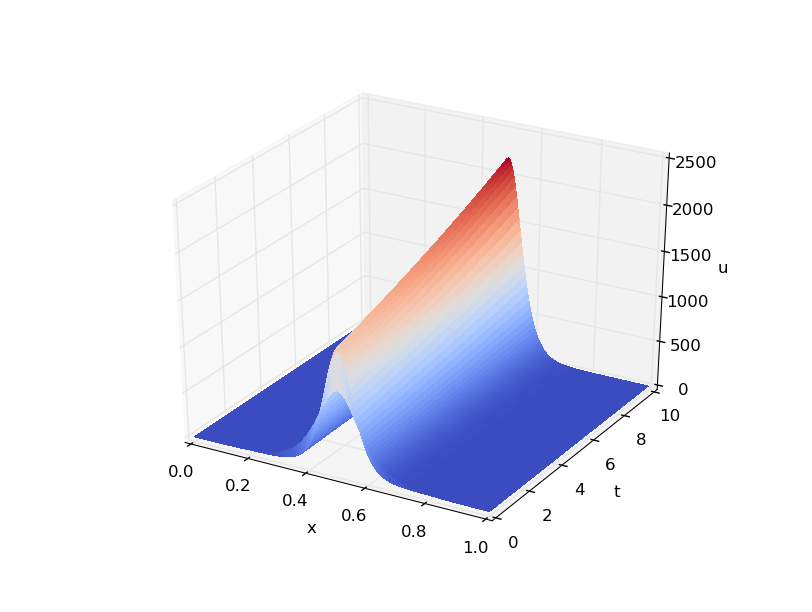
\includegraphics[width=4in]{ex_s15}
    \caption{Без управления}
\end{figure}

\begin{exmp_bur}
\end{exmp_bur}
Теперь начальное условия $\theta_0(x) = \frac{x^2}{G(x)}$. Параметр $\sigma = 15$. 

\begin{figure}[H]
    \centering
    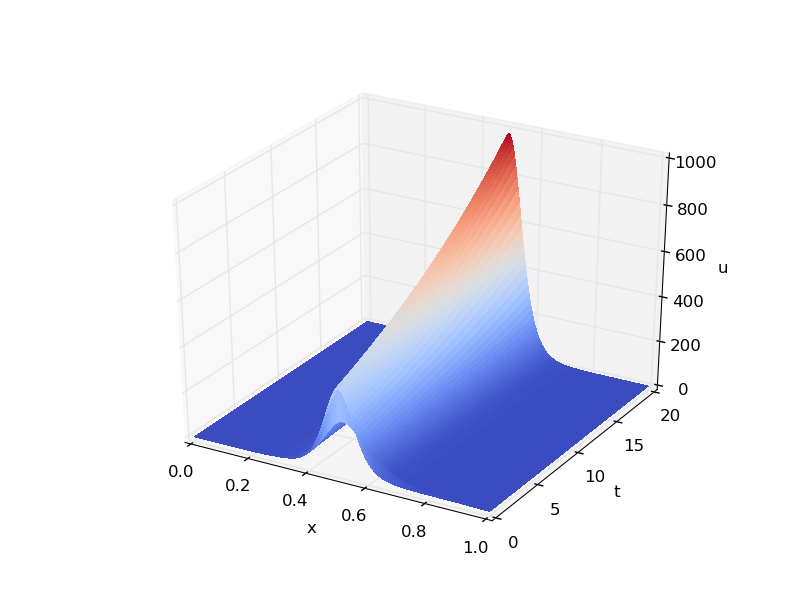
\includegraphics[width=4in]{ex_x2_s15}
    \caption{Без управления}
\end{figure}
